\chapter{Referencial Teórico}

O objetivo desse capítulo é referenciar as teorias que embasam o conteúdo desse trabalho bem como o estado da arte no uso do HOG.

\section{Histograma orientado a gradientes}
\label{sec:HOG}

HOG (Histogram of oriented gradients) é um descritor computado a partir dos gradientes da imagem. Podemos defini-lo como sendo uma informação estatística do gradiente e intensidade de uma área. Suas principais propriedades são a robustez para pequenas variações nos locais dos contornos, direções e variações significativas na iluminação e cor. Na figura \ref{fig:hog} temos um resumo das principais etapas do cálculo feito para extrair o vetor de características.

Na primeira etapa temos uma normalização do gama da imagem para eliminar, de forma global, efeitos nas variações de luminosidade. Depois é aplicado um filtro para o cálculo do gradiente da imagem, resultando em cada pixel, um vetor cuja amplitude e direção representa as variações de intensidade de luz, ou seja, temos como resultado as bordas da imagem. Em seguida a imagem é dividida em uma grade uniforme de células, onde para cada célula um histograma de orientação do gradiente é calculado. As células são finalmente agrupadas em blocos e normalizadas gerando assim um vetor de características que será a concatenação dos histogramas normalizados de cada bloco.

\begin{figure}[ht!]
\centering
\fbox{
  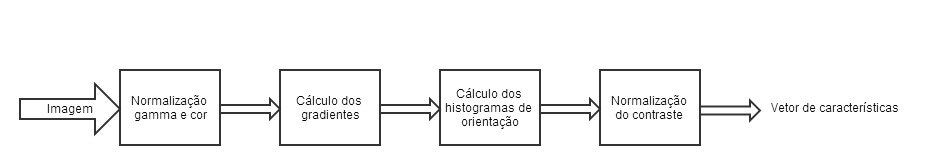
\includegraphics[scale=0.5]{image/hog.jpg}}
  \caption{Fluxo de cálculo para extrair o vetor de características}
  \label{fig:hog}
\end{figure}

Para usar como referência, daqui para adiante vamos nos referir ao conjunto de parâmetros do HOG usado pelo \citeonline{dalal2005histograms} para detecção de pessoas como sendo o HOG original.

% Colocar no final de cada texto a referência do Dalal.
% Adicionar em cada final de secao um previa do proximo.

\subsection{Normalização Gama/Cor}

Os pixeis de uma imagem podem ser representados de diversas maneiras como escala de cinza, RGB e LAB. Quando disponível, a informação de cor sempre ajuda a aumentar a performance do descritor, mas a sua representação em RGB ou LAB possuem performances semelhantes.
Uma equalização da luminância (correção gama) ainda pode ser opcionalmente aplicado para reduzir a influência dos efeitos da iluminação de uma maneira global. A correção gama, nos casos mais simples, é definida conforme equação \ref{eq:power_law}. Onde \(A\) é uma constante e os valores de entrada e saída são valores reais não negativos. \cite{dalal2005histograms}

\begin{equation}
V_{out} = AV_{in}^\gamma
\label{eq:power_law}
\end{equation}

Na figura \ref{fig:gamma_correction} tem-se um exemplo de diversos valores para o valor de gama para uma imagem da base de dados. Em (a) o gama de valor 2 realça as cores mais escuras, em (b) a imagem se mantém como a original, sem alterações. Em (c) e (d), com gama de valor \(1/2\) e \(1/3\) respectivamente, temos um realce dos tons mais claros.

\begin{figure}[ht!]
\centering
  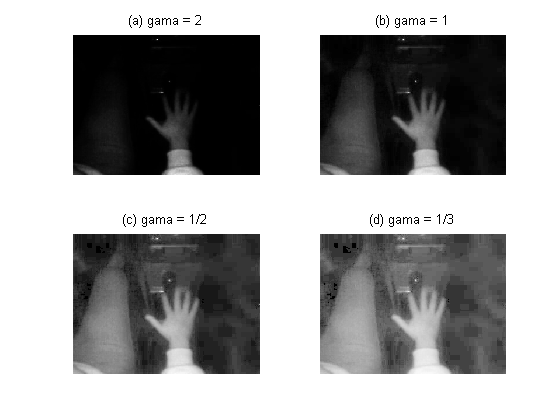
\includegraphics[scale=0.8]{image/gamma_correction.png}
  \caption{Exemplificação para valores diferentes de gama}
  \label{fig:gamma_correction}
\end{figure}

Depois da normalização do gama, a imagem está pronta para ser filtrada e ter seus gradientes calculados.

\subsection{Gradientes}

Um dos mais importantes processos no processamento de uma imagem é a sua segmentação. A segmentação consiste em subdividir a imagem em regiões ou objetos de interesse. O nível de segmentação depende do problema a ser resolvido e é comumente baseado em duas propriedades do valor da intensidade: descontinuidade e similaridade. A primeira consiste em particionar uma imagem com base nas mudanças abruptas de intensidade, como por exemplo as bordas de um objeto. Já na segunda, é feito o agrupamento de uma região com base em sua similaridade com outras partes da imagem, como cor ou nível de intensidade.

\citeonline{gonzalez2002digital} definem borda como sendo um conjunto de pixeis conectados  presente na fronteira entre duas regiões. E conclui que a magnitude da primeira derivada pode ser usada para detectar a borda em um ponto da imagem.

A derivada de primeira ordem de uma imagem digital pode ser aproximada no gradiente 2D. O gradiente de uma imagem \(f(x,y)\) no ponto \((x,y)\) e definido como um vetor

\begin{equation}
\nabla \mathbf{f}(x,y) = 
\begin{bmatrix}
G_x \\ G_y
\end{bmatrix} =
\begin{bmatrix}
\dfrac{ \partial f}{\partial x} 
\\[2ex]
\dfrac{ \partial f}{\partial y}
\end{bmatrix}
\end{equation}

cuja magnitude é definida como \(\nabla f\), onde

\begin{equation}
\nabla f = mag(\nabla \mathbf{f}) = 
\begin{bmatrix}
G_x^2 + G_y^2
\end{bmatrix}^{1/2}
\label{eq:mag}
\end{equation}

e a direção do vetor \(\alpha(x,y)\) sendo definida como

\begin{equation}
\alpha(x,y) = tan^{-1}
\left (
\dfrac{G_y}{G_x}
\right)
\end{equation}

onde o ângulo é medido em referência ao eixo \(x\). A direção de uma borda no ponto \((x,y)\) é perpendicular à direção do vetor gradiente no ponto.

O cálculo dessas derivadas pode ser implementado usando máscaras como o da figura \ref{fig:gradiente_mascara}. A máscara é aplicada em cada pixel da imagem e um novo valor é calculado conforme a equação \ref{eq:gradiente_mascara}.

\begin{equation}
R = w_1 z_1 + w_2 z_2 + w_3 z_3 + ... +w_9 z_9 = \sum_{i=1}^{9}{w_iz_i}
\label{eq:gradiente_mascara}
\end{equation}

\begin{figure}
\begin{center}
\begin{tabular}{| l |c | r |}
\hline
\(w_1\) & \(w_2\) & \(w_3\) \\ \hline
\(w_4\) & \(w_5\) & \(w_6\) \\ \hline
\(w_7\) & \(w_8\) & \(w_9\) \\ \hline
\end{tabular}
\end{center}
\caption{Exemplo de máscara 3x3}
\label{fig:gradiente_mascara}
\end{figure}

\begin{figure}
	\centering
	\begin{subfigure}[b]{0.3\textwidth}
	\begin{center}
		\begin{tabular}{| l | c | r |}
		\hline
		-1 & -1 & -1 	\\ \hline
		0 & 0 & 0 		\\ \hline
		1 & 1 & 1 		\\ \hline
		\end{tabular}
		\begin{tabular}{| l | c | r |}
		\hline
		-1 & 0 & 1	 	\\ \hline
		-1 & 0 & 1 		\\ \hline
		-1 & 0 & 1 		\\ \hline
		\end{tabular}
		\caption{Máscara Prewitt}
		\label{fig:gradiente_prewitt}
	\end{center}
	\end{subfigure}
	\begin{subfigure}[b]{0.3\textwidth}
	\begin{center}
		\begin{tabular}{| l | c | r |}
		\hline
		-1 & -2 & -1 	\\ \hline
		0 & 0 & 0 		\\ \hline
		1 & 2 & 1 		\\ \hline
		\end{tabular}
		\begin{tabular}{| l | c | r |}
		\hline
		-1 & 0 & 1	 	\\ \hline
		-2 & 0 & 2 		\\ \hline
		-1 & 0 & 1 		\\ \hline
		\end{tabular}
		\caption{Máscara Sobel}
		\label{fig:gradiente_sobel}
	\end{center}
	\end{subfigure}]
	\caption{Exemplo de máscara de gradientes}
\end{figure}

Nas figuras \ref{fig:gradiente_prewitt} e \ref{fig:gradiente_sobel} temos dois exemplos das máscaras mais utilizadas para cálculo de gradiente. Na figura \ref{fig:gradientes} pode-se ver o resultado das máscaras em uma imagem de uma pose de mão fechada feita por uma câmera infravermelha. A figura (a) é a imagem original, (b) e (c) são os resultados da filtragem pela máscara Prewitt em \(x\) e em \(y\). A figura (d) mostra a magnitude do vetor de gradiente depois da filtragem pela máscara Prewitt. As figuras (e) e f) são os resultados da filtragem pela máscara Sobel em \(x\) e em \(y\), e (g) é a magnitude do vetor de gradiente depois da filtragem pela máscara Sobel.

\begin{figure}
    \centering
    \begin{subfigure}[b]{0.3\textwidth}
        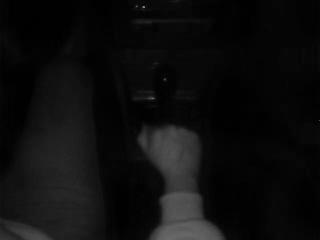
\includegraphics[width=\textwidth]{image/gradiente_original.jpg}
        \caption{Original}
        \label{fig:gradiente_original}
    \end{subfigure}%
    ~ %add desired spacing between images, e. g. ~, \quad, \qquad, \hfill etc.
      %(or a blank line to force the subfigure onto a new line)
    \begin{subfigure}[b]{0.3\textwidth}
        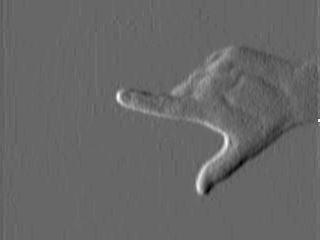
\includegraphics[width=\textwidth]{image/gradiente_prewitt_gx.jpg}
        \caption{Prewitt Gx}
        \label{fig:gradiente_gx}
    \end{subfigure}
    ~ %add desired spacing between images, e. g. ~, \quad, \qquad, \hfill etc.
      %(or a blank line to force the subfigure onto a new line)
    \begin{subfigure}[b]{0.3\textwidth}
        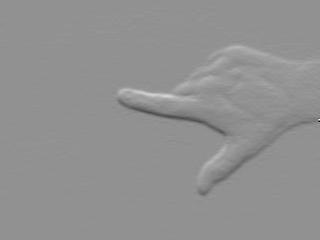
\includegraphics[width=\textwidth]{image/gradiente_prewitt_gy.jpg}
        \caption{Prewitt Gy}
        \label{fig:gradiente_gy}
    \end{subfigure}
    \begin{subfigure}[b]{0.3\textwidth}
        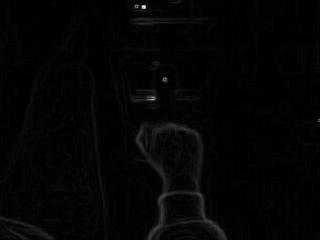
\includegraphics[width=\textwidth]{image/gradiente_prewitt_mag.jpg}
        \caption{Prewitt Gmag}
        \label{fig:gradiente_gmag}
    \end{subfigure}%
    ~ %add desired spacing between images, e. g. ~, \quad, \qquad, \hfill etc.
      %(or a blank line to force the subfigure onto a new line)
    \begin{subfigure}[b]{0.3\textwidth}
        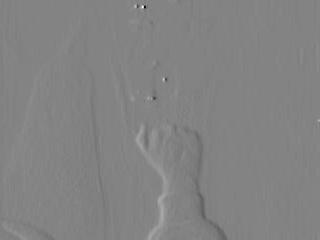
\includegraphics[width=\textwidth]{image/gradiente_sobel_gx.jpg}
        \caption{Sobel Gx}
        \label{fig:gradiente_gx}
    \end{subfigure}
    ~ %add desired spacing between images, e. g. ~, \quad, \qquad, \hfill etc.
      %(or a blank line to force the subfigure onto a new line)
    \begin{subfigure}[b]{0.3\textwidth}
        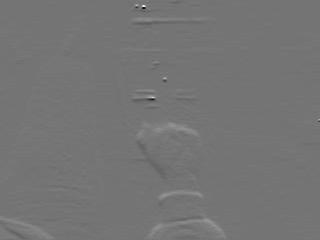
\includegraphics[width=\textwidth]{image/gradiente_sobel_gy.jpg}
        \caption{Sobel Gy}
        \label{fig:gradiente_gy}
    \end{subfigure}
    \begin{subfigure}[b]{0.3\textwidth}
        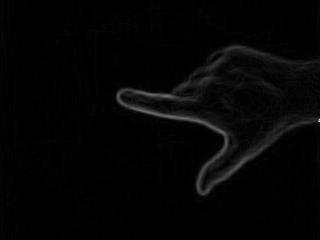
\includegraphics[width=\textwidth]{image/gradiente_sobel_mag.jpg}
        \caption{Sobel Gmag}
        \label{fig:gradiente_gmag}
    \end{subfigure}
    \caption{Gradientes}\label{fig:gradientes}
\end{figure}

No HOG original a máscara usada é uma máscara centrada 1-D [-1 0 1]. O gradiente é computado da seguinte maneira: \cite{dalal2005histograms}

\begin{equation}
	G_{x}(x,y) = f(x+1, y) - f(x-1, y)
\end{equation}
\begin{equation}
	G_{y}(x,y) = f(x, y+1) - f(x, y-1)
\end{equation}

Com a imagem filtrada, já é possível fazer o cálculo dos histogramas.

\subsection{Cálculo dos histogramas}

Para o cálculo dos histogramas, a imagem é então dividida em pequenos retângulos (células). Para cada célula, um histograma é calculado. Esse histograma é a coleção dos ângulos dos vetores de gradiente de cada pixel que compõe a célula. Cada pixel apresenta um peso na construção do histograma das orientações das bordas. Esse peso pode ser em função do gradiente, do seu quadro ou da sua raiz.

Os ângulos podem ser agrupados variando de 0 á 360 graus ou de 0 á 180 graus.

No HOG original, as células tem tamanho 8x8, as orientações são ponderadas pela magnitude do vetor e uniformemente agrupas em 9 grupos de 0 á 180 graus. \cite{dalal2005histograms}

O processo de cálculo do histograma descrito é conceitual e possui detalhes de implementação que devem ser levados em consideração conforme apêndice D do \citeonline{dalal2006finding}.

\subsection{Normalização em blocos}

%The first stage applies an optional global image normalisation equalisation that is de-signed to reduce the influence of illumination effects. In practice we use gamma (power
%law) compression, either computing the square root or the log of each colour channel.
%Image texture strength is typically proportional to the local surface illumination so this
%compression helps to reduce the effects of local shadowing and illumination variations.

O tamanho do gradiente pode variar bastante por conta de variações como iluminação e contraste entre o fundo e o objeto de interesse. Portanto, um importante passo para se obter um bom resultado na extração do vetor de características do objeto é a sua normalização.

Norma é uma função que atribui um tamanho de valor positivo e diferente de zero para um vetor em um espaço vetorial.

A função norma deve satisfazer algumas propriedades de escalabilidade e aditividade.
Sendo um espaço vetorial \(V\) em um sub corpo \(F\) de números complexos, a norma em \(V\) é uma função \(p:\rightarrow \mathbf{R}\) com as seguintes propriedades:

\begin{itemize}
\item \( p(a\mathbf{v}) = |a|p(\mathbf{v}) \)
\item \( p(\mathbf{u + v}) \leq p(\mathbf{u}) + p(\mathbf{v}) \)
\item Se \( p(\mathbf{v}) = 0 \) então \(\mathbf{v}\) é o vetor zero.
\end{itemize}

Uma norma bastante usada é a norma euclidiana,  que diz que em um espaço euclidiano \(R^n\) a norma será:

\[\|x\| := \sqrt{x_1^2 + ... + x_n^2}\]

Dos vários esquemas de normalização, a maioria é baseada no agrupamento de células em blocos maiores e normalizando o contraste de cada bloco separadamente. Além disso, há uma sobreposição entre blocos para que as células de cada bloco possam contribuir nas componentes de normalização diversas vezes. Quatro esquemas foram testados por Dalal, sendo \(v\) um vetor não normalizado, \(||v||_k\) sua \(k-norm\) para \(k=1,2\) e \(\epsilon\) uma constante pequena temos:

\begin{itemize}
\item L2-norm, \(v \to \frac{v}{\sqrt{||v||_2^2 + \epsilon^2}}\);
\item L2-Hys, L2-norm seguido por uma limitação nos valores máximos de \(v\) em 0.2 e renormalizando; 
\item L1-norm, \(v \to \frac{v}{||v||_1 + \epsilon}\);
\item L1-sqrt, \(v \to \sqrt{\frac{v}{\sqrt{||v||_2^2 + \epsilon^2}}}\).
\end{itemize}

Cada bloco normalizado gera um vetor de características locais. O resultado final como descritor da imagem é a concatenação desses blocos.

O HOG proposto por \citeonline{dalal2005histograms} possui parametrização conforme tabela \ref{table:dlal_hog}. Ela é o resultado do estudo do melhor conjunto de parâmetros para a extração do vetor de características usando essa técnica para pessoas. 

\begin{table}[!h]
\centering
\begin{tabular}{|c|c|}
\hline Cor & RGB sem correção de gamma \\ 
\hline Gradiente & [-1, 0, 1] sem smoothing \\ 
\hline Bins & 9 \\
\hline Orientação & 0 à 180 \\
\hline Tamanho do bloco & 16x16 pixels \\
\hline Tamanho da célula & 8x8 pixels \\
\hline Normalização & L2-Hys \\
\hline Janela de detecção & 64x128 \\
\hline 
\end{tabular} 
\caption{Parâmetros do HOG otimizado por \citeonline{dalal2005histograms} para detecção de humanos}
\label{table:dlal_hog}
\end{table}

\section{Estado da arte}

% % % % % % % % % % % % % % % % % % % % % % % % % % % % % % % %
% Orientation histograms for hand gesture recognition
% 1995 / Japão / Mitsubishi
% Computer vision for computer games
% 1996 / Japão / Mitsubishi
Um dos precursores em extração de características da mão usando histograma de orientação de gradientes foi o laboratório da Mitsubishi que publicou um conjunto de artigos \cite{freeman1995orientation, freeman1996computer} sobre o tema. Com o objetivo de identificar poses e gestos de mão para interfacear com aplicativos e jogos de computador, a abordagem foi aplicar o cálculo de um histograma de orientações de gradiente na imagem convertendo-a em um vetor de características, que depois era comparado com um outro vetor de características de uma base de treinamento usando a distância euclidiana. Com apenas o cálculo de um histograma, o sistema apresentava vetor de características muito parecidas para poses diferentes e exigia que a mão dominasse a área da imagem. Em imagens onde o tamanho da mão não era significativo (como a imagem de uma pessoa de corpo inteiro), a mudança da pose tinha pouco impacto no histograma.

% % % % % % % % % % % % % % % % % % % % % % % % % % % % % % % %
% Distinctive Image Features from Scale-Invariant Keypoints
Foi na elaboração do SIFT em \cite{lowe2004distinctive}, que o uso da técnica do histograma de orientação de gradientes ficou genérico para diversas aplicações e acabou se tornando popular. O SIFT usa o vetor de gradiente de pontos chaves da imagem para gerar seu vetor de característica, mas a vantagem do método se dá na normalização em blocos que aumenta o desempenho do algoritmo. Ele é conhecido por um algoritmo para detectar e descrever características locais da imagem. O algoritmo é patenteado nos Estados Unidos pela Universidade da Colúmbia Britânica.

% % % % % % % % % % % % % % % % % % % % % % % % % % % % % % % %
% Histograms of Oriented Gradients for Human Detection
Em \cite{dalal2005histograms} uma combinação com os histogramas de orientações de gradientes já existentes com a metodologia de normalização em blocos similar ao \cite{lowe2004distinctive} foi proposta como descritor para seres humanos. O alto desempenho do método fez com que a metodologia aplicada no trabalho se tornasse referência para quando se fala em HOG.  Esse artigo é a base desse trabalho e cada etapa e parâmetro do algoritmo são discutidos em \ref{sec:HOG}. Além de calibrar os parâmetros para obter uma melhor performance na detecção de pessoas, os autores ainda os comparam com outros três métodos existentes de descritores (Haar wavelets, PCA-SIFT e shape context) mostrando a boa performance do método.

% % % % % % % % % % % % % % % % % % % % % % % % % % % % % % % %
% An Effective Crossing Cyclist Detection on a Moving Vehicle 
Em \cite{li2010effective} o HOG é utilizado para a detecção de ciclistas. No método proposto não foi feito overlap no cálculo dos histogramas, como uma maneira de melhorar o tempo de processamento, a amostragem piramidal é utilizada para extrair características globais em diferentes escalas. As imagens utilizadas são em tons de cinza e um filtro gaussiano é aplicado antes do cálculo dos HOGs (contrariando as orientações do \citeonline{dalal2005histograms}). O gradiente é calculado com máscara [-1 0 +1], os ângulos são calculados entre 0 e 180, e o histograma é dividido em 20 grupos de ângulos. A imagem é dividida em blocos de 16x16 sem divisão de células. O classificador utilizado é um SVM linear. Esse trabalho é interessante pois propõe um método para melhorar a velocidade do cálculo dos histogramas, o que pode ser útil para aplicações em tempo real embarcadas.

% % % % % % % % % % % % % % % % % % % % % % % % % % % % % % % %
% Hand-gesture recognition: comparative study of global, semi-local and local approaches
Um estudo comparando descritores locais, semi locais e globais é feito em \cite{collumeau2011hand}. O objetivo do trabalho é estudar qual seria o método mais adequado para descrever poses de mão em uma sala de cirurgia para que o médico possa enviar comandos para os aparelhos sem precisar encostar neles. Para descritores globais foram usado os momentos de Zernike (invariante em rotação, translação e escala) combinados com um classificador linear SVM. O HOG é usado como um descritor semi local e SIFT para locais. Apesar de não dar detalhes de como são feitos os cálculos do HOG, o artigo mostra uma melhor performance do método. No melhor resultado encontrado, a taxa de reconhecimento do HOG foi de 87,66\%, contra 73,32\% do Zernike e 69,32\% do SIFT.

% % % % % % % % % % % % % % % % % % % % % % % % % % % % % % % %
% A vision-based system for automatic hand washing quality assessment
Nesse artigo \cite{llorca2011vision}, o problema a ser resolvido era verificar, com o uso de uma câmera, se uma pessoa  fez as seis diferentes poses de mão para o lavar correto das mãos. Primeiro as imagens são segmentadas por cor de pele e depois um estimador de posição do braço e da mão baseado em um filtro multi modal probabilístico é proposto. Um ROI é criado com o resultado do filtro anterior e então HOG é aplicado, usando como classificadores dois SVM independentes. Um para o HOG normal e outro para o HOF (Histogram of optical flow). Essa combinação espacial e temporal melhorou o desempenho do sistema aumentando a taxa de detecção.

% % % % % % % % % % % % % % % % % % % % % % % % % % % % % % % %
% Automatic Ship Recognition Robust Against Aspect Angle Changes and Occlusions
Nesse artigo \cite{kawahara2012automatic}, é utilizado a coHOG (co-occurence HOG) para reconhecimento de navios em imagens ISAR. Cinco navios diferentes foram testados em ângulos de 0\degree, 30\degree e 60\degree, e com oclusão da popa. No coHOG os blocos, durante a normalização, são agrupados em pares. Esse agrupamento causa um aumento na dimensão do vetor de características que o deixa robusto para imagens em diferentes ângulos e na oclusão.

% An Extended HOG Model: SCHOG for Human Hand Detection
% 2012 / China
% [1, 2] Verificar o que são essas referências
% [7] Ler referência, o texto cita essa referência como o básico para HOG.
% O porque usar SVM [11, 12]
%Nesse artigo o HOG é modificado para funcionar nas cores de pele. Usou apenas o gesto de palma aberta.	

% % % % % % % % % % % % % % % % % % % % % % % % % % % % % % % %
% A ROBUST METHOD OF FINGERTIP DETECTION IN COMPLEX BACKGROUND
A abordagem do artigo \cite{jiang2012robust} é criar um método para detectar as pontas dos dedos de uma mão de palma aberta com um câmera localizada em um óculos. A mão a ser detectada é a do próprio usuário do óculos, portanto as imagens serão de cima da mão. Um ângulo bastante semelhante ao do trabalho dessa pesquisa. Primeiramente a região da mão é encontrada usando o HOG como descritor e o SVM como classificador e posteriormente uma abordagem geométrica utilizando convex hull é aplicada para achar as pontas dos dedos. Os parâmetros utilizados para o cálculo do HOG foram células de 12x12 pixeis, com blocos de 2x2 células, ângulos variando de 0 a 180 graus agrupados em 9 regiões. Esse trabalho é uma boa referência de que o HOG pode ser utilizado para encontrar uma região de interesse com alta probabilidade de se ter uma mão, mas infelizmente ele só abrange uma pose de mão.

% Deformable HOG-based Shape Descriptor
% 2013 - Espanha	
% [8] - Referência à HOG do artigo
%A escrita a mão são compostas por região de pouca informação e outra com informação concentrada. A divisão feita normalmente pelo HOG é uma divisão rígida que não permite focar nas regiões de %maior interesse.

% % % % % % % % % % % % % % % % % % % % % % % % % % % % % % % %
% Gesture Components for Natural Interaction with In-Car devices &
% Gesture control for use in auto-mobiles
Em \cite{zobl2004gesture} e em \cite{akyol2000gesture} tem-se um cenário automotivo idêntico ao proposto, no qual imagens infravermelhas de uma câmera instalada no teto do carro são capturadas e traduzidas em gestos e poses de mão. Em \cite{zobl2004gesture} o sistema proposto pelo artigo é capaz de reconhecer onze gestos e quatro poses. A imagem capturada com resolução 384x144 é primeiramente processada com uma combinação de subtração de fundo e threshold global. Em \cite{akyol2000gesture} é usado apenas um threshold global. A mão é considerada o maior objeto da cena. Depois da segmentação, um filtro para retirar o braço é aplicado e finalmente são calculados os momentos da imagem, para o cálculo da área e do centro de massa, e os momentos Hu. Usar os momentos Hu como vetor de características limita bastante a aplicação pois sua pose é representada por apenas 7 dimensões, o que parece um tanto quanto insuficiente. E a aproximação de que a mão é o maior objeto da cena é bem irreal, pois podemos ver, na base de dados extraída nessa pesquisa, que constantemente a perna do motorista ou o painel do veículo são os objetos maiores da cena.

% % % % % % % % % % % % % % % % % % % % % % % % % % % % % % % %
% Real-time Vision-based Infotainment User Determination for Driver Assistance
% % % % % % % % % % % % % % % % % % % % % % % % % % % % % % % %
% Hand Gesture to Control Infotainment Equipment in Cars
Em \cite{cheng2008real} e em \cite{parada2014hand} temos também o uso de câmeras infra vermelha no teto do carro. O primeiro tem o objetivo de discriminar quem está usando o painel de controles do carro, o motorista ou o passageiro, e assim adaptar os controles para aumentar a segurança. O motorista, quando usa o sistema de multimídia, tem a opção de controles reduzida para evitar distrações. Nesse estudo a posição do ROI é fixa e dividida em uma grade de células 2x2, o histograma é calculado para cada célula com 8 grupos de ângulos variando de 0 á 360 graus, portanto formando um vetor de 32 dimensões. O tamanho do ROI também é analisado variando entre 140x80, 80x80 e 140x140. O sistema faz uso de um classificador SVM e possui uma taxa de 96.8\% de acerto. Esse trabalho mostra uma alta taxa de acerto usando um vetor de características de apenas 32 dimensões, mostrando um bom potencial para aplicações de tempo real.

Já o segundo tem a proposta de identificar poses e gestos para comandar o sistema multimídia do veículo. Para isso é feita uma combinação de remoção de fundo para segmentação e geometria computacional para classificação da pose. A segmentação é o resultado de três algoritmos rodando em paralelo, o Edge-based Foreground-Background Model (EBM), Mixture of Gaussians background Model (BG\_MoG) e Maximally Stable Extremal Regions segmenter (MSER). Essa estratégia resulta em um modelo para remoção de fundo estático e dinâmico, permitindo uma pré calibração do fundo com imagens estáticas e também se adaptando a eventuais mudanças por conta de novos objetos, sombras e diferentes condições de luminosidade.

% % % % % % % % % % % % % % % % % % % % % % % % % % % % % % % %
% Gesture-Based Automotive Controls
% 2012 - Google
O Google em \cite{hobbs2012gesture} também tem mostrado interesse no reconhecimento de gestos no interior de veículos. Em sua patente, ele diz que o ar condicionado, os vidros e o rádio podem ser controlados por gestos que serão mapeados por câmeras de profundidade. A patente não especifica quais gestos ou quais algoritmos devem ser usados, mas já mostra que a gigante, que hoje já possui um carro autônomo totalmente funcional, está mirando seus esforços para a interação homem - veículos através de gestos.